\documentclass{article}

\usepackage{lastpage}
\usepackage{fancyhdr} % Required for custom headers
\usepackage{extramarks} % Required for headers and footers
\usepackage[usenames,dvipsnames]{color} % Required for custom colors
\usepackage{graphicx} % Required to insert images
\usepackage{subcaption}
\usepackage{listings} % Required for insertion of code
\usepackage{color}
\usepackage{rotating}
\usepackage{courier} % Required for the courier font
% Below are optional packages
\usepackage{amsmath}
\usepackage{amssymb}
\usepackage{float}
\usepackage{pdfpages}
\usepackage{multirow}
\usepackage{algorithm}
\usepackage{algorithmic}
\usepackage{hyperref}

% Margins
\topmargin=-0.45in
\evensidemargin=0in
\oddsidemargin=0in
\textwidth=6.5in
\textheight=9.0in
\headsep=0.25in

\linespread{1.1} % Line spacing

% Set up the header and footer
\pagestyle{fancy}
\lhead{\hmwkAuthorNameOne , \hmwkAuthorNameTwo} % Top left header
\chead{\hmwkTitle} % Top center head
\rhead{\hmwkClass} % Top right header
\lfoot{\lastxmark} % Bottom left footer
\cfoot{} % Bottom center footer
\rfoot{Page\ \thepage\ of\ \protect\pageref{LastPage}} % Bottom right footer
\renewcommand\headrulewidth{0.4pt} % Size of the header rule
\renewcommand\footrulewidth{0.4pt} % Size of the footer rule

\setlength\parindent{0pt} % Removes all indentation from paragraphs

% Define Colors for Code Snippets in Java
\definecolor{dkgreen}{rgb}{0,0.6,0}
\definecolor{gray}{rgb}{0.5,0.5,0.5}
\definecolor{mauve}{rgb}{0.58,0,0.82}

\lstset{frame=tb,
  language=C++,
  aboveskip=3mm,
  belowskip=3mm,
  showstringspaces=false,
  columns=flexible,
  basicstyle={\small\ttfamily},
  numbers=none,
  numberstyle=\tiny\color{gray},
  keywordstyle=\color{blue},
  commentstyle=\color{dkgreen},
  stringstyle=\color{mauve},
  breaklines=true,
  breakatwhitespace=true,
  tabsize=4
}

\newcommand{\cpp}{\lstinline[language=C++]}
%------------------------------------------------------------------------------------
%   DOCUMENT STRUCTURE COMMANDS
%   Skip this unless you know what you're doing
%------------------------------------------------------------------------------------

% Header and footer for when a page split occurs within a problem environment
\newcommand{\enterProblemHeader}[1]{
    %\nobreak\extramarks{#1}{#1 continued on next page\ldots}\nobreak
    %\nobreak\extramarks{#1 (continued)}{#1 continued on next page\ldots}\nobreak
}

% Header and footer for when a page split occurs between problem environments
\newcommand{\exitProblemHeader}[1]{
    %\nobreak\extramarks{#1 (continued)}{#1 continued on next page\ldots}\nobreak
    %\nobreak\extramarks{#1}{}\nobreak
}

\setcounter{secnumdepth}{0} % Removes default section numbers
\newcounter{homeworkProblemCounter} % Creates a counter to keep track of the number of problems
\setcounter{homeworkProblemCounter}{0}

\newcommand{\homeworkProblemName}{}
\newenvironment{homeworkProblem}[1][Part \arabic{homeworkProblemCounter}]{ % Makes a new environment called homeworkProblem which takes 1 argument (custom name) but the default is "Problem #"
    \stepcounter{homeworkProblemCounter} % Increase counter for number of problems
    \renewcommand{\homeworkProblemName}{#1} % Assign \homeworkProblemName the name of the problem
    \section{\homeworkProblemName} % Make a section in the document with the custom problem count
    \enterProblemHeader{\homeworkProblemName} % Header and footer within the environment
}{
    \exitProblemHeader{\homeworkProblemName} % Header and footer after the environment
}

\newcommand{\problemAnswer}[1]{ % Defines the problem answer command with the content as the only argument
    \noindent\framebox[\columnwidth][c]{\begin{minipage}{0.98\columnwidth}#1\end{minipage}} % Makes the box around the problem answer and puts the content inside
}

\newcommand{\homeworkSectionName}{}
\newenvironment{homeworkSection}[1]{ % New environment for sections within homework problems, takes 1 argument - the name of the section
    \renewcommand{\homeworkSectionName}{#1} % Assign \homeworkSectionName to the name of the section from the environment argument
    \subsection{\homeworkSectionName} % Make a subsection with the custom name of the subsection
    \enterProblemHeader{\homeworkProblemName\ [\homeworkSectionName]} % Header and footer within the environment
}{
    \enterProblemHeader{\homeworkProblemName} % Header and footer after the environment
}


%=================================================================

%------------------------------------------------------------------------------------
%   NAME AND CLASS SECTION
%------------------------------------------------------------------------------------

\newcommand{\hmwkTitle}{MapReduce Implementation of Google's PageRank Algorithm} % Assignment title
\newcommand{\hmwkSubtitle}{using MPI} % Assignment Subtitle
\newcommand{\hmwkClass}{COL380} % Course/class
\newcommand{\hmwkClassTitle}{Introduction to Parallel and Distributed Computing} % Course/class title
\newcommand{\hmwkAuthorNameOne}{Vasu Jain} % Your name
\newcommand{\hmwkAuthorNameTwo}{Shreya Sharma} % Your name
\newcommand{\hmwkEntryNumberOne}{2017CS10387} % Your entry number
\newcommand{\hmwkEntryNumberTwo}{2017CS50493} % Your entry number


%------------------------------------------------------------------------------------
%   TITLE PAGE
%------------------------------------------------------------------------------------

\title{
    \textmd{\hmwkClass :\ \hmwkClassTitle}\\
    \vspace{2in}
    \textmd{\textbf{\hmwkTitle}}\\
    \textmd{\hmwkSubtitle}\\
    % \normalsize\vspace{0.1in}\small{Due\ on\ \hmwkDueDate}\\
    \vspace{3in}
}
        
\author
{
    \textbf{\hmwkAuthorNameOne:\ \hmwkEntryNumberOne}
    \ ,
    \textbf{\hmwkAuthorNameTwo:\ \hmwkEntryNumberTwo}
}

% Insert date here if you want it to appear below your name
\date{\today} 

%------------------------------------------------------------------------------------

\begin{document}
    
    \maketitle
    \clearpage
    \tableofcontents
    \clearpage
    
    %=========================================================
    %   Data Structure and Algorithm Optimization: 
    %=========================================================
    \section{Design Philosophy, Objectives and Workflow}
    
    We approached this assignment with the following objectives and design philosophy:
    \begin{enumerate}
        \item Implement mapreduce-pagerank using mapreduce C++ library
        \item Implement our own mapreduce library with MPI by implementing  the functions needed for pagerank. 
        \item  Implement pagerank using existing mapreduce MPI library.
    In each of the above cases compare correctness of the pagrank output against the given java/python outputs.
        \item Plot graphs with x-axis as benchmark ID, and y-axis as pagerank runtime (three graphs for the three executables).
        \item Compare pagerank latencies across the three implementations and comment on the observations
    \end{enumerate}
    The time measurements were done by using the \cpp{std::chrono::high_resolution_clock} 
    % and code was compiled with -O3 Optimization flag.
    These objectives were achieved to a large extent by continuous evolution of the code-base.
    The design philosophy caused changes across the objectives in tandem. However, the general design cycle was \\
    
    Optimize Serial $\longrightarrow$ Parallelize algorithm $\longrightarrow$ Refactor Code $\longrightarrow$ Optimize Serial $\longrightarrow$ ... \\
    
    Our code and scripts can be found in the repository at:
    {\newline}
    \url{https://github.com/jainvasu631/MPI-MapReduce-PageRank}
    % \clearpage
    
    %=========================================================
    %   Mapreduce Algorithm
    %=========================================================
    \section{The PageRank Algorithm}
    We will assign to each web page P a measure of its importance I(P), called the page's PageRank.

    Suppose that page Pj has lj links. If one of those links is to page Pi, then Pj will pass on 1/lj of its importance to
    Pi. The importance ranking of Pi is then the sum of all the contributions made by pages linking to it. That is, if we denote the set of pages linking to Pi by Bi, then I({P_i})=\sum{\frac{I(P_j)}{l_j}},   {P_j\in B_i}
    % \newline 
    
    \begin{itemize}
        \item \textbf{Hyperlink Matrix} \newline
        H := [Hij] = if Pj in Bi then 1/lj else 0 \newline
        H := [Hij] = if Pj to Pi is Edge then 1/lj else 0 \newline
        H is a \textbf{stochastic matrix}. The sum of all entries in a column is 1/0
        
        \item \textbf{Importance Vector} \newline
        I := [I(Pi)] whose components are the PageRanks or the importance rankings of all the pages.\newline
        I = HI i.e. I is an eigenvector of H with eigenvalue 1. This is the \textbf{stationary vector} of H.
        
        \item \textbf{Computing I} \newline
        H can be a very very large matrix of the order of $10^10$. However most entries of H are zero.Therefore its a sparse matrix. \newline
        I(k+1) = HI(k). Sequence of I(k) converges to I.

    \end{itemize}
    
    \subsection{Problems with Convergence of I}
    \begin{enumerate}
        \item Dangling nodes which have no out links. Then H is no more perfectly stochastic. In this case these nodes will act as importance sinks.
        \item Circular Reference Problem. S isn't Primitive anymore and the I(k) never converges.
        \item Importance Sink. S is reducible, i.e. when we have a sub graph of fully connected nodes with no edge coming out of it.
    \end{enumerate}
    
    \subsection{Solving the Problem}
    \subsubsection{Google Matrix}
    Replace all 0 columns in matrix H with 1/n to create S. Thus we don't have dangling nodes anymore. \newline
    So, S = H + A where A := [Aij] = {if Hi==0 then 1/n else 0} \newline
    \newline
    Choose a parameter $\alpha$ between 0 and 1. Now, with probability $\alpha$ , the random surfer is guided by S and with probability $ 1-\alpha $ , he chooses the next page at random. This solves the problem of importance sinks and circular references.  \newline
    So, G := $\alpha$ x S + $(1-\alpha)$ x 1/n x 1.
    \subsubsection{Choosing alpha}
    The parameter $\alpha$ has an important role. When $\alpha$ is 1 we get G:=S and when $\alpha$ is 0 G:=$(1-\alpha)$/n x 1. The rate of convergence of I depends on $\alpha$. Therefore as a compromise we use $\alpha$ = 0.85.
    
    \subsection{Optimizing the Calculation}
    \subsubsection{Simplifying Formula}
    I(k+1) = $\alpha$ x H x I(k) + $\alpha$ x A x I(k) + $(1-\alpha)$/n x 1 x I(k). \newline
    This can be further simplified. A = J/n where J = [Ji] = {1 if Corresponding Column is 0 else 0}.\newline
    Let  $\beta$ := (1/$\alpha$-1) and so M:= (J + $\beta$ x 1)/n.  \newline
    Then I(k+1) = $\alpha$ x (H x I(k) + (J + (1/$\alpha$-1) x 1)/n x I(k)) which simplifies to \newline
    I(k+1) = $\alpha$ (H I(k) + M I(k)).
    \subsubsection{Calculating M x I(k)}
    As all rows of M are identical, we can write M = 1 x N and M x I(k) = 1 x N x I(k).  \newline
    factor:= N x I(k) = (1 + beta if Corresponding column is 0 else beta) x I(k)/n
    \newline Now the expression simplifies to 
    I(k+1) = $\alpha$ x H x I(k) + 1 x factor.  
    \clearpage
    
    %=========================================================
    %   Data Structure and Algorithm Optimization: 
    %=========================================================
    \section{Data Structures}
    \subsection{Graphs}
    Input files contain two space separated numbers (denoting 2 web-pages) in each line indicating a link from the first webpage to the second. We read and convert the input into a graph with # of nodes (N) = maximum node index in the file.
    
    Class Graph contains - 
    \begin{itemize}
        \item VertexList (type vector(int))- Protected variable denoting a list of vertices (type int).
        \item EdgeList (type vector(pair(int,int))) - Protected variable denoting list of edges (type pair(int,int)).
        \item toList (type vector(VertexList)) - Public variable denoting a list such that toList[i] is the VertexList of all the vertices which have an edge from "i".
        \item fromList (type vector(VertexList)) - Public variable denoting a list such that fromList[i] is the VertexList of all the vertices which have an edge to "i".
    \end{itemize}{}
    
    \subsection{Columns}
    Columns is a vector of Values where Values has type - "double". Two important uses of Columns are -
    \begin{itemize}
        \item PageRank - This data structure simply contains the calculated page rank for each web-page.
        \item Hyperlink - ith element of Hyperlink contains the importance ith node will give to the nodes it has an outgoing edge to.
    \end{itemize}
    \subsection{Initialization}
    After the graph is generated from the input file:
    \begin{lstlisting}[caption={ Calculating Hyperlink}] 
        static Column calculateHyperLinkColumn(const Graph::ToList& toList){
            const Graph::Size N = toList.size();
            Column hyperlink(N);
            for(Graph::Size i=0;i<N;i++)
                hyperlink[i] = (toList[i].size()>0)? 1.0/toList[i].size() : 0;
            return hyperlink;
        }
    \end{lstlisting}
    PageRank is initialised as a vector of doubles of size N with all values = 1.0/N
    \begin{lstlisting}[caption={ Initialising PageRank}] 
        static inline Column getInitPageRank(const Graph::Size N) {
            return Column(N,1.0/N);
        }
    \end{lstlisting}
 
    
    % \subsubsection{Time Complexity Analysis}
    % The 2 parts have serial time complexity:
    % \begin{enumerate}
    %     \item Initialization - $O(N^2)$ (Quadratic due to Initialization of A and B by random numbers)
    %     \item Matrix Multiplication - $O(N^2)$ (Quadratic due to the 2 nested for loops of Size N in matrix multiplication side the main loop. The third innermost loop is of constant size as M=32)
    %     \item Checking Correctness - $O(N^2)$ ( Quadratic due to iterating over all elements of two $N\times N$ \cpp{FlatMatrix})
    % \end{enumerate}
    
    \clearpage
    %=========================================================
    %   Mapreduce C++ Library
    %=========================================================
    \section{Mapreduce C++ Library}
    The MapReduce C++ Library implements a single-machine platform for programming using the the Google MapReduce idiom. Users specify a map function that processes a key/value pair to generate a set of intermediate key/value pairs, and a reduce function that merges all intermediate values associated with the same intermediate key. 
    
    The developer is required to write two classes:
    \begin{itemize}
        \item MapTask - It implements a mapping function to process key/value pairs generate a set of intermediate key/value pairs 
        \item ReduceTask - It implements a reduce function to merges all intermediate values associated with the same intermediate key. 
    \end{itemize}
    There are three optional template parameters that can be used to modify the default implementation:
    \begin{itemize}
        \item Datasource - It implements a mechanism to feed data to the Map Tasks - on request of the MapReduce library
        \item Combine - It can be used to partially consolidate results of the Map Task before they are passed to the Reduce Tasks
        \item IntermediateStore - It handles storage, merging and sorting of intermediate results between the Map and Reduce phases
    \end{itemize}{}
    
    \subsection{Our Implementation}
    We have used the concept of Mapreduce while solving the pagerank finding problem at two steps. First is in finding the factor Column (as defined in the pagerank algorithm section) and second is in finding the pagerank Column.
    \subsubsection{Calculating Factor using Mapreduce}
    \begin{lstlisting}[caption={ MapTask for Factor}] 
        class MapFactor : public mapreduce::map_task<Graph::Vertex, Value>{
            // Identity Map
            public: template<typename Runtime>
                void operator()(Runtime& runtime, const key_type& key, const value_type& value) const{runtime.emit_intermediate(COMMON,value);}
            private: static constexpr Graph::Size COMMON = 0;              
        };
    \end{lstlisting}
    
    \begin{lstlisting} [caption = {ReduceTask for Factor}]
        class ReduceFactor : public mapreduce::reduce_task<Graph::Size, Value>{
            // Calculate Factor by Accumulation
            public: template<typename Runtime, typename Iterator>
                void operator()(Runtime& runtime, const key_type& key, Iterator it, Iterator end) const{runtime.emit(key,std::accumulate(it,end,0.0));}
        };
    \end{lstlisting}
    
    We have defined a class named FactorData used by "Calculation" - an instance of mapreduce::job to compute factor column using mapreduce template of C++.
    
    \begin{lstlisting} [caption = {Mapreduce Job for Factor}]
        using Calculation = mapreduce::job<MapFactor,ReduceFactor, mapreduce::null_combiner,FactorData>;
    \end{lstlisting}
    
    
    \subsubsection{Calculating PageRank using Mapreduce}
    
    \begin{lstlisting}[caption={ MapTask for PageRank}] 
        class MapPageRank : public mapreduce::map_task<Graph::Vertex, VertexInfo >{
            // Function to generate Intermediate Values
            // Will map for each to Vertex a probability contribution that is summed by reduce      
            public: template<typename Runtime>
                void operator()(Runtime& runtime, const key_type& key, const value_type& value) const{
                    runtime.emit_intermediate(key, ZERO); // Emitting Zero Insures that each Node has atleast Tuple
                    for (const Graph::Vertex& to : value.second) 
                        runtime.emit_intermediate(to, value.first);
                }
            private: static constexpr Value ZERO = 0.0;              
        
        };
    \end{lstlisting}
    
    \begin{lstlisting} [caption = {ReduceTask for PageRank}]
        class ReducePageRank : public mapreduce::reduce_task<Graph::Vertex, Value>{
            // Function to add all probabilities in Hyperlink Matrix        
            public: template<typename Runtime, typename Iterator>
                void operator()(Runtime& runtime, const key_type& key, Iterator it, Iterator end) const{runtime.emit(key,std::accumulate(it,end,0.0));}
        };
    \end{lstlisting}
    
    We have defined a class named PageRankData used by "Iteration" - an instance of mapreduce::job to compute pageRank column using mapreduce template of C++.
    
    \begin{lstlisting} [caption = {Mapreduce Job for PageRank}]
        using Iteration = mapreduce::job<MapPageRank, ReducePageRank, mapreduce::null_combiner,PageRankData>;
    \end{lstlisting}
    
    \clearpage
    %=========================================================
    %   Self-implemented Mapreduce Library using MPI
    %=========================================================
    \section{Self-implemented Mapreduce Library using MPI}

    
    \clearpage
    
    %=========================================================
    %   Mapreduce MPI Library
    %=========================================================
    \section{Mapreduce MPI Library}
    
    \subsection{In terms of Principle}
     In C++, your program includes two library header files and uses the MapReduce namespace: \newline
     \newline
        \textbf{#include "mapreduce.h" \newline
        #include "keyvalue.h"   \newline
        using namespace MAPREDUCE\_NS   \newline}
        
    Arguments to the library's \textbf{map()} and \textbf{reduce()} methods include function pointers to serial "mymap" and "myreduce" functions in your code (named anything you wish), which will be "called back to" from the library as it performs the parallel map and reduce operations. \newline \newline
    A typical simple MapReduce program involves these steps: 
    
    \begin{lstlisting} [caption = {MapReduce Program Layout}]
        MapReduce *mr = new MapReduce(MPI_COMM_WORLD); // instantiate an MR object
        mr->map(nfiles,&mymap); // parallel map
        mr->collate() // collate keys
        mr->reduce(&myreduce); // parallel reduce
        delete mr; // delete the MR object
    \end{lstlisting}
    
    All the library methods operate on two basic data structures stored within the MapReduce object -
    \begin{itemize}
        \item
         \textbf{KeyValue object (KV)} - A KV is a collection of key/value pairs. The same key may appear many times in the collection, associated with values which may or may not be the same. 
        \item
        \textbf{KeyMultiValue object (KMV)} - A KMV is also a collection of key/value pairs. But each key in the KMV is unique, meaning it appears exactly once.The value associated with a KMV key is a concatenated list (a multi-value) of all the values associated with the same key in the original KV.
    \end{itemize}
     
     Various library methods operated on KV and KMV objects in our implementation are - 
     \begin{itemize}
         \item \textbf{MapReduce add() method} - \textit{uint64\_t MapReduce::add(MapReduce *mr2)} \newline
         Adds the KeyValue pairs contained in a second MapReduce object mr2, to the KeyValue object of the first MapReduce object, which is created if one does not exist. 
         
         \item \textbf{MapReduce broadcast() method} - \textit{uint64\_t MapReduce::broadcast(int root) } \newline
         Deletes the key/value pairs of a KeyValue object on all processors except root, and then broadcasts the key/value pairs owned by the root processor to all the other processors.
         
         \item \textbf{MapReduce collate() method} - \textit{uint64\_t MapReduce::collate(int (*myhash)(char *, int))  } \newline
         Aggregates a KeyValue object across processors and converts it into a KeyMultiValue object. 
         
         \item \textbf{MapReduce gather() method} - \textit{uint64\_t MapReduce::gather(int nprocs)  } \newline
         Collects the key/value pairs of a KeyValue object spread across all processors to form a new KeyValue object on a subset (nprocs) of processors. 
         
         \item \textbf{MapReduce sort\_keys() method} - \textit{uint64\_t MapReduce::sort\_keys(int flag)   } \newline
         Sorts a KeyValue object by its keys to produce a new KeyValue object. 
         
     \end{itemize}
    
    \clearpage
    
    \subsection{In terms of Implementation}  
    
    The concept of approach is completely similar to the one used in the first part with MapReduce C++ Library. We calculate the factor column and then the pagerank column using MapReduce API of MPI. 
    
    \subsubsection{Calculating Factor using Mapreduce of MPI}
    \begin{lstlisting}[caption={ "mymap" function for Factor}] 
        static void MapFactor(Graph::Vertex key, KeyValue* keyvalue, void* calculator){
            Value value = castTo(Calculator,calculator)->getFactorValue(key);
            auto Common = COMMON;
            keyvalue->add(getCharAddress(Common),VERTEX_SIZE,getCharAddress(value),VALUE_SIZE);
        }
    \end{lstlisting}
    
    \begin{lstlisting} [caption = { "myreduce" function for Factor}]
        static void ReduceFactor(char* key, int keybytes, char* multivalue, int nvalues, int* valuebytes, KeyValue* keyvalue, void* calculator){ 
            // cout << ((nvalues==0)? "Trouble" : "Phew") <<endl;
            Value* values = castTo(Value,multivalue);    
            Value factor = accumulate(values,values+nvalues,0.0)/nvalues;
            keyvalue->add(key, VERTEX_SIZE,getCharAddress(factor),VALUE_SIZE);
        }
    \end{lstlisting}

    \begin{lstlisting} [caption = { "mygather" function for Factor}]
        static void GatherFactor(uint64_t index, char* key, int keybytes, char* value, int valuebytes, KeyValue* keyvalue, void* calculator)
        { castTo(Calculator,calculator)->factor = dereferenceTo(Value,value); } // Replace Factor
        }
    \end{lstlisting}
    
    \begin{lstlisting} [caption = {Calculating Factor}]
        auto kvPairs = mapreduce.map(N,MapFactor,void_this);// Map Part
        mapreduce.collate(NULL);
        auto kvmPairs = mapreduce.reduce(ReduceFactor,void_this);// Reduce Part
        mapreduce.gather(HOME);
        mapreduce.broadcast(ROOT);
        kvPairs = mapreduce.map(&mapreduce,GatherFactor,void_this);// Gather Part
    \end{lstlisting}
    
    Similarly to Calculate Pagerank
    
    \clearpage
    
    %=========================================================
    %   Performance Analysis 
    %=========================================================
    \section{Performance Analysis}
    
    % For the Blocking and Non-Blocking Communication there is no restriction on the input matrix size dimension 'N' and the number of threads in the MPI\_Communication - 'SIZE'. 
    % \begin{itemize}
    %         \item When 'N' is a multiple of 'SIZE' we simply give CHUNK\_SIZE = (N/SIZE) number of rows of matrix 'A' to each thread to compute CHUNK\_SIZE number of rows of the output matrix. 
    %         \item When 'N' is a not a multiple of 'SIZE' we give CHUNK\_EXTRA = (N\%SIZE) number of rows of matrix 'A' to the last ranked thread in addition to the CHUNK\_SIZE rows to compute (CHUNK\_SIZE + CHUNK\_EXTRA) rows of matrix 'C'.
    %     \end{itemize}    
    
    % In case of Collective communication when 'N' is a multiple of 'SIZE' we divide the work between the threads just like we do in Blocking and Non-blocking. But when 'N' is a not a multiple of 'SIZE', we compute the CHUNK\_EXTRA = (N\%SIZE) number of rows of output matrix 'C' in the process of root thread itself and parllelize the computation of all the remaining (N - CHUNK\_EXTRA) rows of 'C' just like the case when 'N' is a multiple of 'SIZE'. 
    
    % \clearpage
    
    %=========================================================
    %   Experimental Observations of Execution Time: 
    %   Explanation of the findings and trends of graph in accordance with the theoretical time complexity: 
    %=========================================================
    \section{Observations and Conclusions}
    \subsection{Execution Time of Different Implementations}
    \newline \newline
   \includegraphics [scale=0.65] {Table2_Mapreduce.png}
    
    \subsection{Time Complexity Analysis}
    
    % \begin{figure}[H]
    %     \centering
    %     \begin{subfigure}[H]{\linewidth}
    %         \centering
    %         \includegraphics[width=0.6\linewidth]{Images/Blocking_Parallel_Execution_Time_vs_N.png}
    %         \caption{Blocking Matrix Multiplication}
    %     \end{subfigure}
    %     \begin{subfigure}[H]{\linewidth}
    %         \centering
    %         \includegraphics[width=0.6\linewidth]{Images/Non_Blocking_Parallel_Execution_Time_vs_N.png}
    %         \caption{Non Blocking Matrix Multiplication}
    %     \end{subfigure}
    %     \begin{subfigure}[H]{\linewidth}
    %         \centering
    %         \includegraphics[width=0.6\linewidth]{Images/Collective_Parallel_Execution_Time_vs_N.png}
    %         \caption{Collective Matrix Multiplication}
    %     \end{subfigure}
        
    %     \caption{Matrix Multiplication Time Complexity for Different Number of Threads}
    %     \label{fig:0}
    % \end{figure}
    
    \clearpage
    
    \subsection{Observations and Explanations of Graph Trends}
    
    \subsubsection{MapReduce C++ Library}
    \begin{enumerate}
        \item Benchmark - Barabasi
        \begin{center}
            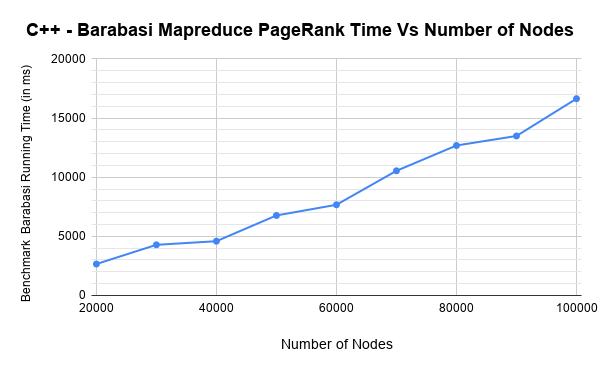
\includegraphics[scale = 0.6]{C++ - Barabasi Mapreduce PageRank Time Vs Number of Nodes.png}
        \end{center}
            
        
        \item Benchmark - Erdos
        \begin{center}
            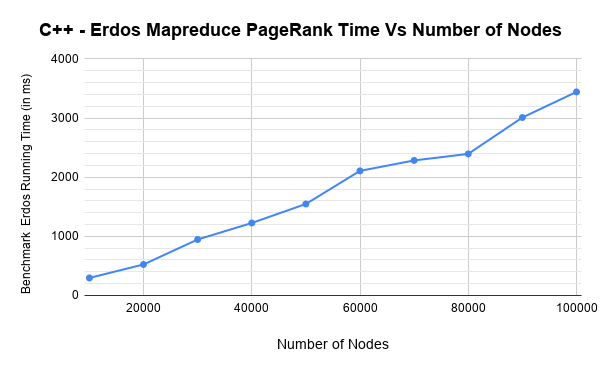
\includegraphics[scale = 0.6]{C++ - Erdos Mapreduce PageRank Time Vs Number of Nodes.png}
        \end{center}
    \end{enumerate}
    
    \clearpage
    
    \subsubsection{MapReduce Self with MPI}
    \begin{enumerate}
        \item Benchmark - Barabasi
        \begin{center}
            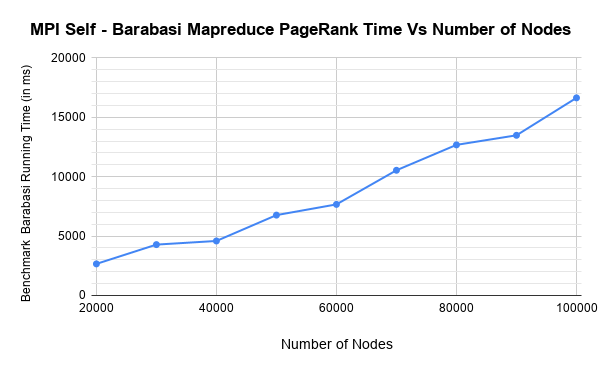
\includegraphics[scale = 0.6]{MPI Self - Barabasi Mapreduce PageRank Time Vs Number of Nodes.png}
        \end{center}
            
        
        \item Benchmark - Erdos
        \begin{center}
            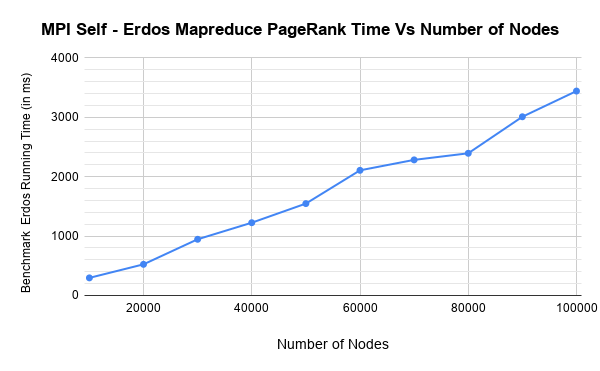
\includegraphics[scale = 0.6]{MPI Self - Erdos Mapreduce PageRank Time Vs Number of Nodes.png}
        \end{center}
    \end{enumerate}
    
    \clearpage
    
    \subsubsection{MapReduce with MPI Library}
    
    \begin{enumerate}
        \item Benchmark - Barabasi
        \begin{center}
            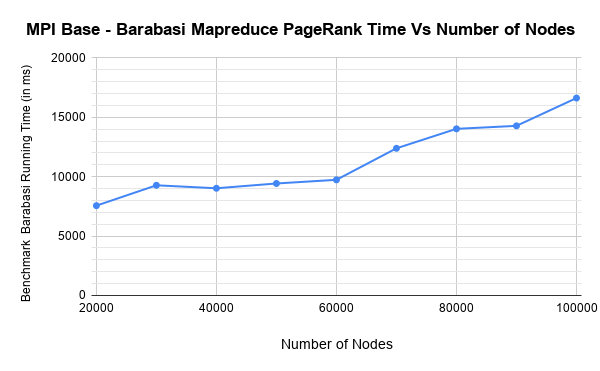
\includegraphics[scale = 0.6]{MPI Base - Barabasi Mapreduce PageRank Time Vs Number of Nodes.png}
        \end{center}
            
        
        \item Benchmark - Erdos
        \begin{center}
            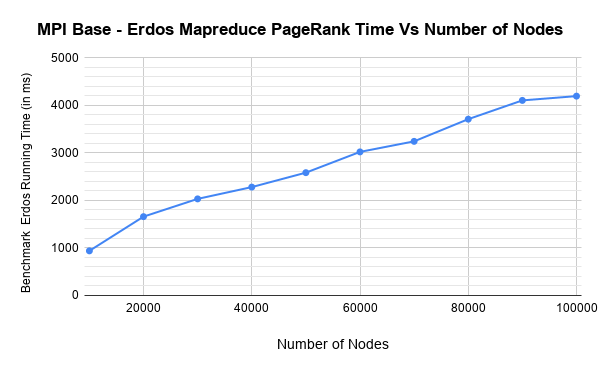
\includegraphics[scale = 0.6]{MPI Base - Erdos Mapreduce PageRank Time Vs Number of Nodes.png}
        \end{center}
    \end{enumerate}
    
    \clearpage
    
    \
    
    % \begin{enumerate}
    %     \item We also observe that speedup is around 1.2-2.1X when going from 1 Thread to 2 Threads and 3.1-3.3X when going to 4 Threads in Case of Blocking and Collective Matrix Multiplication. 
    %     \item However beyond 4 Threads the speedup doesn't increase further and efficiency nose dives. 
    %     This is due to the Quad Core nature of the Processor used in the experiments and it doesn't provide a significant speedup when going beyond 4 threads or processes (i.e its processor count).
    %     In fact there can be a penalty to the context switching done in higher number of threads (8 and 16). 
    %     \item The efficiency hovers between 0.7-1 when 1,2 and 4 threads are used but nosedives when more threads are used.
    %     \item We also observed that Execution Time of Blocking and Collective Communication were close to each other with Blocking being around 2-10\% faster. However this gap became relatively smaller for bigger problem sizes.
    %     \item We also observed that Execution Time of Non Blocking is much slower and speedup is significantly less than and Collective Communication were close to each other with Blocking being around 2-10\% faster. This gap increase as problem size increases.
    %     \item Another observation is that at smaller problem sizes of N=1000, speedup and efficiency are lower but they increase slowly as problem sizes goes to N=8000.
    % \end{enumerate}
    
    
    %=========================================================
    %   End
    %=========================================================
    
\end{document}
